% This file was created with tikzplotlib v0.10.1.
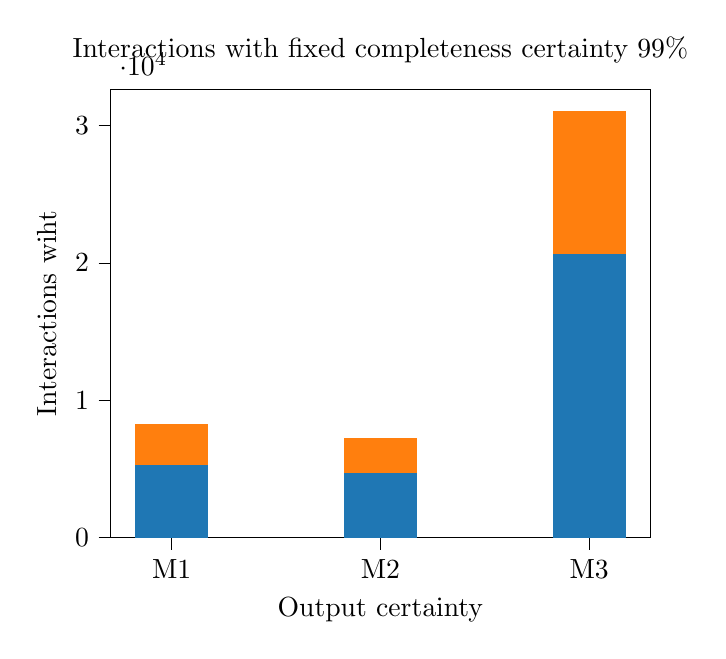
\begin{tikzpicture}

\definecolor{darkgray176}{RGB}{176,176,176}
\definecolor{darkorange25512714}{RGB}{255,127,14}
\definecolor{lightgray204}{RGB}{204,204,204}
\definecolor{steelblue31119180}{RGB}{31,119,180}

\begin{axis}[
legend cell align={left},
legend style={
  fill opacity=0.8,
  draw opacity=1,
  text opacity=1,
  at={(0.03,0.97)},
  anchor=north west,
  draw=lightgray204
},
tick align=outside,
tick pos=left,
title={Interactions with fixed completeness certainty  99\%},
x grid style={darkgray176},
xlabel={Output certainty },
xmin=-0.2925, xmax=2.2925,
xtick style={color=black},
xtick={0,1,2},
xticklabels={M1,M2,M3},
y grid style={darkgray176},
ylabel={Interactions wiht \SUL},
ymin=0, ymax=32626.65,
ytick style={color=black}
]
\draw[draw=none,fill=steelblue31119180] (axis cs:-0.175,0) rectangle (axis cs:0.175,5257);
\draw[draw=none,fill=steelblue31119180] (axis cs:0.825,0) rectangle (axis cs:1.175,4677);
\draw[draw=none,fill=steelblue31119180] (axis cs:1.825,0) rectangle (axis cs:2.175,20620);
\draw[draw=none,fill=darkorange25512714] (axis cs:-0.175,5257) rectangle (axis cs:0.175,8257);
\draw[draw=none,fill=darkorange25512714] (axis cs:0.825,4677) rectangle (axis cs:1.175,7251);
\draw[draw=none,fill=darkorange25512714] (axis cs:1.825,20620) rectangle (axis cs:2.175,31073);
\path [draw=black, semithick]
(axis cs:0,5257)
--(axis cs:0,5257);

\path [draw=black, semithick]
(axis cs:1,4677)
--(axis cs:1,4677);

\path [draw=black, semithick]
(axis cs:2,20620)
--(axis cs:2,20620);

\path [draw=black, semithick]
(axis cs:0,8257)
--(axis cs:0,8257);

\path [draw=black, semithick]
(axis cs:1,7251)
--(axis cs:1,7251);

\path [draw=black, semithick]
(axis cs:2,31073)
--(axis cs:2,31073);

\end{axis}

\end{tikzpicture}
